% Figure: rotating one line through k accounts (Proposition 4).
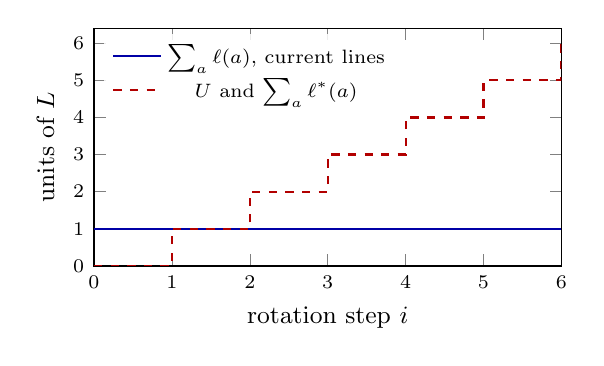
\begin{tikzpicture}
  \begin{axis}[
      width=0.62\linewidth, height=4.6cm,
      xmin=0, xmax=6, ymin=0, ymax=6.4,
      xlabel={rotation step $i$}, ylabel={units of $L$},
      xtick={0,...,6}, ytick={0,...,6},
      legend style={font=\scriptsize, at={(0.02,0.98)}, anchor=north west, draw=none, fill=white, fill opacity=0.85, text opacity=1},
      tick label style={font=\scriptsize}, label style={font=\small},
    ]
    \addplot[const plot, thick, blue!65!black] coordinates {(0,1) (1,1) (2,1) (3,1) (4,1) (5,1) (6,1)};
    \addlegendentry{$\sum_a \ell(a)$, current lines}
    \addplot[const plot, thick, red!70!black, dashed] coordinates {(0,0) (1,1) (2,2) (3,3) (4,4) (5,5) (6,6)};
    \addlegendentry{$U$ and $\sum_a \ell^*(a)$}
  \end{axis}
\end{tikzpicture}
